\chapter{Lezione 11 - Architettura di un Enterprise Content Management System}

Gli argomenti che affronteremo sono un quadro di insieme dell'architettura, la raccolta dei contenuti, la loro gestione, l'archiviazione, la collaborazione dei vari attori e la distribuzione dei contenuti.

Argomenti trattati:

\FloatBarrier
\begin{figure}[H]
  \centering
  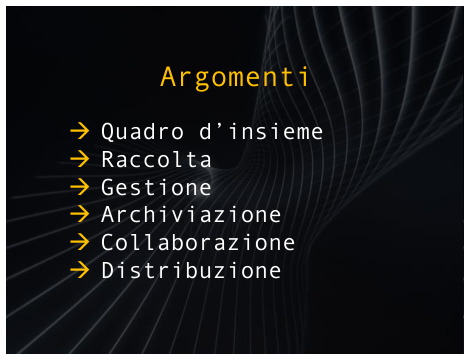
\includegraphics[width=0.50\textwidth,
                    trim=40 60 40 60, % L B R T
                    clip]
                    {images/Lez11_p01_fig_02}
  % \caption{Sommario}
  % \label{fig:Lez15_p06_fig_02}
\end{figure}
\FloatBarrier
\noindent


\section{Quadro di insieme}

\FloatBarrier
\begin{figure}[H]
  \centering
  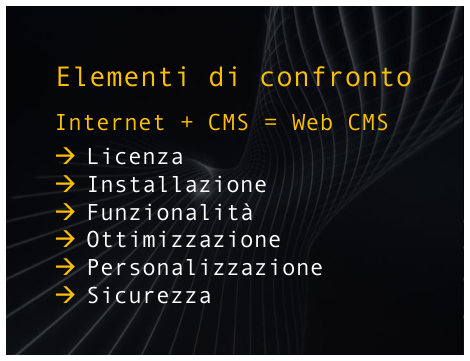
\includegraphics[width=0.50\textwidth,
                    trim=40 40 40 60, % L B R T
                    clip]
                    {images/Lez11_p01_fig_04}
  % \caption{Sommario}
  % \label{fig:Lez15_p06_fig_02}
\end{figure}
\FloatBarrier
\noindent

Esiste una grande varietà di sistemi per la gestione dei contenuti estesa anche dalla possibilità di consultazione e di presentazione dei contenuti nel web.

Vediamo alcuni elementi di confronto.

Il primo criterio è la licenza.

Questi sistemi possono avere una licenza libera, cioè libero uso, libera consultazione, non sono a pagamento.
Oppure avere una licenza open source che permette con determinati vincoli abbastanza laschi la possibilità di modificare, di estendere, di correggere, di personalizzare il sorgente, quindi adattare il sistema alle proprie necessità o eventualmente estendendo con nuovi moduli.

Poi esistono le licenze proprietarie o a pagamento.

Un altro criterio riguarda il tipo di installazione.
Ne sono individuate tre.

Off the shelf, il sistema viene scaricato e installato dove si decide, quindi in casa oppresso un provider.
L'installazione sarà self-hosted, quindi autogestita se viene scaricato e gestito in casa, quindi siamo i fornitori di questo servizio di content management o hosted se ci si appoggia a un altro fornitore.

Le funzionalità sono l'insieme delle operazioni, delle attività che sono supportate automaticamente dal sistema.

L'ottimizzazione che è supportata da attività quali la compressione delle pagine, la pulizia della memoria da documenti o dati obsoleti, piuttosto che alterati, piuttosto che non più validi, il controllo delle sessioni native, l'attivazione di azioni temporizzate, quali per esempio la pubblicazione automatica di documenti, piuttosto che la loro copertura dopo un tempo determinato, e il surchanging optimization, quindi l'ottimizzazione della presentazione dei documenti per l'utilizzo da parte dei motori di ricerca.

La personalizzazione rispetto alle esigenze dell'utente e la sicurezza delle informazioni, dell'accesso, dalla privacy piuttosto che dai diritti, dai copyright, quindi protezione rispetto a questi due concetti, ma anche protezione tecnologica, da accessi non desiderati o non autorizzati alle informazioni gestite.

\FloatBarrier
\begin{figure}[H]
  \centering
  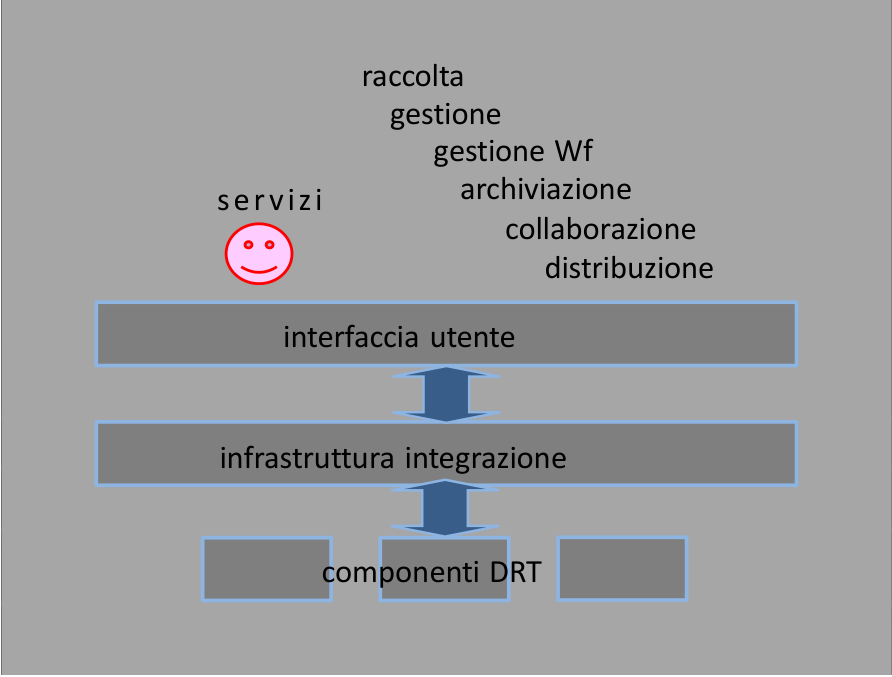
\includegraphics[width=0.60\textwidth,
                    trim=40 30 40 30, % L B R T
                    clip]
                    {images/Lez11_p01_fig_05}
  % \caption{Sommario}
  % \label{fig:Lez15_p06_fig_02}
\end{figure}
\FloatBarrier
\noindent

Vediamo uno schema dell'architettura di un enterprise content management system.

Vi sono tre livelli, a livello basso, i componenti di gestione dei documenti, document related technologies (DRT) che vengono selezionati sulla base delle necessità funzionali dell'organizzazione, integrati con un'apposita struttura di middleware a cui è permesso l'accesso attraverso un'adeguata interfaccia utente che permetta l'accesso uniforme, semplificato e protetto sia per le informazioni, quindi permettendo all'utente di vedere solo le informazioni che è autorizzato a vedere o di sua competenza, sia anche di protezione per eventuali azioni scorrette da parte dell'utente.

L'interfaccia utente offre la possibilità di utilizzare un insieme di servizi per la raccolta delle informazioni, per la gestione dei workflow, quindi l'utente può essere sia utente generico, utente non privilegiato, sia utente amministratore, o utente direzionale del management dell'organizzazione, perché per esempio la gestione del workflow riguarda proprio questo settore.

In seguito i servizi di archiviazione dei contenuti, l'offerta di ambienti o di funzionalità per la collaborazione, per l'interattività e la pubblicazione o copertura dei contenuti o dei documenti, delle pagine, degli articoli che le trasportano.

A questo punto considero completato questo argomento e vi propongo uno spunto di riflessione.
Focalizzate il sistema che utilizzate per la gestione dei contenuti nel vostro ambiente lavorativo o nell'ambiente formativo e provate a descriverlo.
Altro spunto, individuate le sue componenti e le attività che vengono svolte, a un livello di dettaglio che sceglierete voi.

\section{Raccolta dei documenti}

\FloatBarrier
\begin{figure}[H]
  \centering
  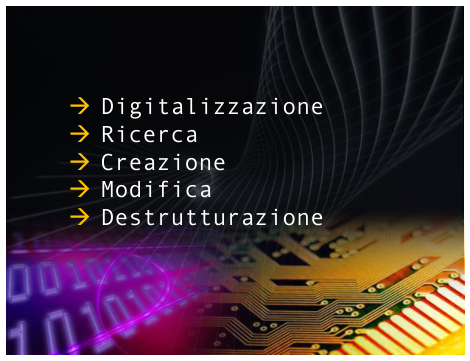
\includegraphics[width=0.50\textwidth,
                    trim=40 100 40 80, % L B R T
                    clip]
                    {images/Lez11_p02_fig_03}
  % \caption{Sommario}
  % \label{fig:Lez15_p06_fig_02}
\end{figure}
\FloatBarrier
\noindent


Cominciamo a descrivere la prima delle attività principali di un enterprise content management system che è la raccolta dei documenti.

La raccolta può essere svolta digitalizzando documenti cartacei, ricercando in rete o accedendo ad altri archivi con documenti già esistenti, oppure producendone di nuovi.

La parte di creazione si estende nella modifica dei documenti esistenti, creandone nuove versioni per correggerli, per aggiornarli o per modificarli strutturalmente.

Altro punto è la destrutturazione dei contenuti.

Per destrutturazione intendiamo lo scomporre un contenuto complesso, un contenuto strutturato in elementi più semplici, in unità più semplici rispetto all'argomento trattato dal contenuto principale.

\FloatBarrier
\begin{figure}[H]
  \centering
  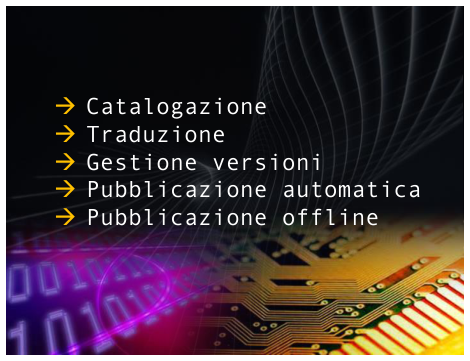
\includegraphics[width=0.50\textwidth,
                    trim=40 100 40 80, % L B R T
                    clip]
                    {images/Lez11_p02_fig_04}
  % \caption{Sommario}
  % \label{fig:Lez15_p06_fig_02}
\end{figure}
\FloatBarrier
\noindent

Una volta acquisiti e preparati i documenti per la sua organizzazione vengono catalogati, quindi vengono prodotte delle descrizioni sintetiche di questi documenti, vengono anche categorizzati per tema, vengono prodotte eventualmente traduzioni o vengono predisposti metadati o strumenti di supporto, tesauri per la loro gestione mediante lingue differenti.

La gestione delle varie versioni è un fatto importante, quindi o le vecchie versioni di un documento che viene nel tempo modificato andranno eliminate per non creare incongruenze nel sistema oppure bisognerà gestirle per riconoscerne le versioni nel tempo e individuare le modifiche ogni volta fatte.

La pubblicazione automatica dei documenti può essere gestita.
La pubblicazione offline vuol dire non pubblicata all'esterno ma solo per il personale di controllo oppure sotto copertura perché le figure addette alla redazione ritengono di proteggere ancora una versione non pronta per la presentazione.

Vi propongo due spunti di riflessione.
Focalizzate ora il sistema che utilizzate per la gestione dei contenuti e individuate quali sono le funzionalità che offre per raccogliere le informazioni.

\section{Gestione dei documenti}

\FloatBarrier
\begin{figure}[H]
  \centering
  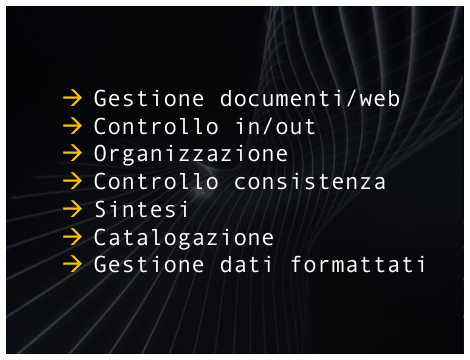
\includegraphics[width=0.50\textwidth,
                    trim=40 60 40 60, % L B R T
                    clip]
                    {images/Lez11_p03_fig_02}
  % \caption{Sommario}
  % \label{fig:Lez15_p06_fig_02}
\end{figure}
\FloatBarrier
\noindent

La gestione riguarda la gestione dei documenti, eventualmente web.
Eventualmente web vuol dire o pagine web, quindi articoli, pagine o documenti, risorse che sono offerte nella rete web.
Quindi accesso ad altri documenti piuttosto che l'offerta di file che possono rappresentare documenti o direttamente pagine web.

La gestione deve includere anche il controllo dell'entrata e dell'uscita di un documento.

Controllo dell'entrata vuol dire protezione da eventuali danneggiamenti del documento piuttosto che dal trasporto di eventuali virus, la correttezza, l'autore, la provenienza, la fonte e l'out vuol dire in caso di documento pubblicato o trasferito va registrato il numero di invii che sono stati effettuati, la data e la versione.

L'organizzazione dei documenti, quindi come sono gestiti in archiviazione sia come strutturazione, come possibilità di accesso, ma anche come eventuale trasporto piuttosto che provvedimenti per il backup, quindi duplicazione.

Il controllo della consistenza, il versioning si occupa proprio di questo, evitare che vi siano versioni non congrue, versioni differenti di documenti, che facciano riferimento allo stesso contenuto.

Possibilità di gestione di sintesi dei documenti attraverso applicativi o funzionalità di mashup che permettono di comporre rapidamente diversi documenti o frammenti di documenti; 
la loro catalogazione, abbiamo visto categorizzazione quindi raggruppamento tematico ma anche produzione di descrizioni sintetiche e la gestione di dati formatati, quindi tratti da database management system che possano essere di supporto a completamento di questi documenti.

Spunto di riflessione: focalizzate il sistema che utilizzate per la gestione dei contenuti e individuate quali sono le funzionalità offerte per l'attività di gestione dei contenuti.

\section{Gestione dei workflow} %14:30

\FloatBarrier
\begin{figure}[H]
  \centering
  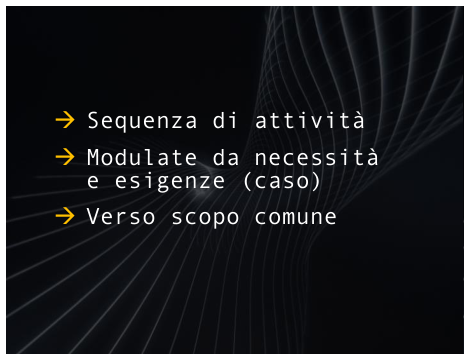
\includegraphics[width=0.50\textwidth,
                    trim=40 100 40 80, % L B R T
                    clip]
                    {images/Lez11_p03_fig_06}
  % \caption{Sommario}
  % \label{fig:Lez15_p06_fig_02}
\end{figure}
\FloatBarrier
\noindent


Per gestione dei workflow indichiamo una sequenza di attività che devono essere svolte, quindi la funzionalità di gestione ci aiuta a individuare queste attività e controllare le regole per il loro corretto svolgimento nell'ordine e nella modalità di esecuzione.

Attività modulate dalla necessità e dalle esigenze, quindi riferite a un caso specifico, a un progetto che deve essere realizzato, un prodotto che deve essere portato a termine o una sequenza di operazioni che c'è stata comandata per raggiungere uno scopo comune, come processo per raggiungere un obiettivo comune a tutti gli attori che partecipano alle attività del workflow.

\FloatBarrier
\begin{figure}[H]
  \centering
  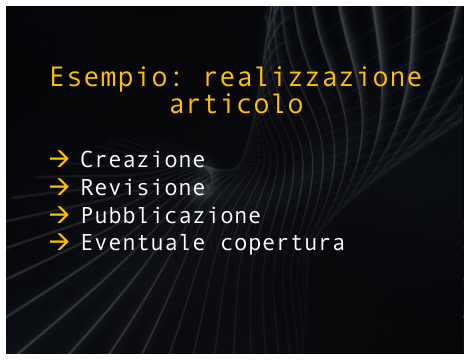
\includegraphics[width=0.50\textwidth,
                    trim=40 80 40 40, % L B R T
                    clip]
                    {images/Lez11_p04_fig_01}
  % \caption{Sommario}
  % \label{fig:Lez15_p06_fig_02}
\end{figure}
\FloatBarrier
\noindent

Consideriamo un esempio nell'ambito editoriale, la realizzazione di un articolo in cui un redattore dovrà occuparsi della parte di creazione, un revisore dovrà verificarne la correttezza, un'ulteriore revisione verrà proposta da un web designer per verificarne la presentazione, la correttezza, il formato; la gestibilità dal sistema verrà verificata da un terzo revisore che è l'amministratore della piattaforma di content management.

A questo punto se il supporto del contenuto, quindi il documento piuttosto che la pagina, piuttosto che l'articolo passano questa revisione, l'articolo potrà essere pubblicato; l'articolo potrà essere messo in coda di pubblicazione, cioè approvato per la pubblicazione, l'articolo verrà pubblicato nella data stabilita, potrà essere pubblicato solo per la consultazione interna oppure anche per la consultazione esterna o potrà a un certo punto anche essere tolto dalla consultazione; quindi eventualmente potrà in seguito essere coperto.

\FloatBarrier
\begin{figure}[H]
  \centering
  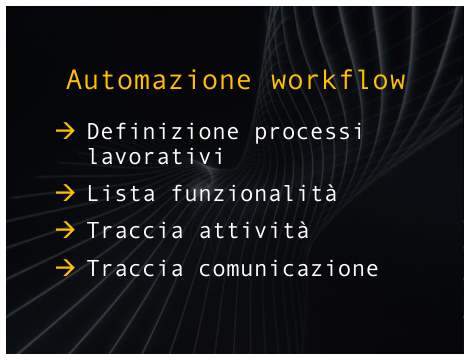
\includegraphics[width=0.50\textwidth,
                    trim=40 60 40 40, % L B R T
                    clip]
                    {images/Lez11_p04_fig_02}
  % \caption{Sommario}
  % \label{fig:Lez15_p06_fig_02}
\end{figure}
\FloatBarrier
\noindent

La gestione automatica di un insieme di attività di questo genere richiede la definizione dei processi lavorativi, quindi dovrà disporre di una lista di funzionalità disponibili, quindi dell'attività componibili in un flusso di lavoro; questa lista di funzionalità non è sempre fornita da un sistema per la gestione dei contenuti.

Dovrà essere fornita la possibilità di tracciare l'attività, quindi monitorare lo svolgimento delle attività per sollecitare o per avvisare dell'attivazione le attività seguenti e memorizzare i risultati intermedi e finali delle varie attività che sono svolte.

Anche la comunicazione deve essere tracciata, sia la comunicazione tra i vari attori durante lo svolgimento del flusso di lavoro, sia anche la comunicazione, lo scambio di messaggi, eventualmente di attivazione effettuato dalle varie attività attivate.

\FloatBarrier
\begin{figure}[H]
  \centering
  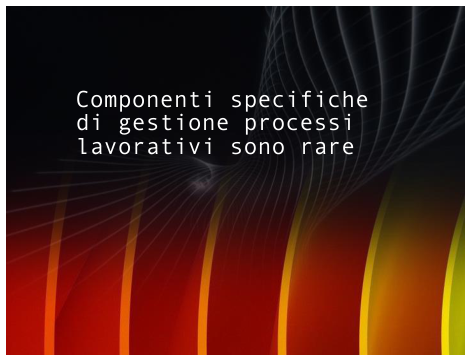
\includegraphics[width=0.50\textwidth,
                    trim=40 150 40 40, % L B R T
                    clip]
                    {images/Lez11_p04_fig_03}
  % \caption{Sommario}
  % \label{fig:Lez15_p06_fig_02}
\end{figure}
\FloatBarrier
\noindent

Come aveva già accennato componenti specifiche di gestione dei processi lavorativi in un content management system sono molto rare, perché la gestione dei processi lavorativi è automatizzata con applicativi piuttosto complessi, quindi costosi e non sempre inclusi come componenti in queste piattaforme.

Alla fine di questo argomento vi propongo una riflessione: focalizzando il sistema che utilizzate per la gestione dei contenuti verificate che permetta la gestione dei flussi di lavoro.


\section{Archiviazione}

\FloatBarrier
\begin{figure}[H]
  \centering
  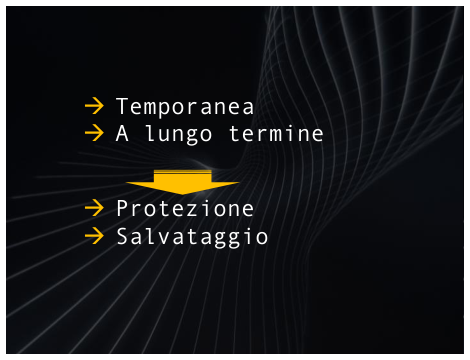
\includegraphics[width=0.50\textwidth,
                    trim=40 80 40 60, % L B R T
                    clip]
                    {images/Lez11_p05_fig_01}
  % \caption{Sommario}
  % \label{fig:Lez15_p06_fig_02}
\end{figure}
\FloatBarrier
\noindent

L'archiviazione può essere temporanea, stiamo parlando di contenuti che hanno una validità temporale ridotta; abbiamo visto per esempio gli interventi in un forum, i commenti in un post, piuttosto che mail, piuttosto che messaggi attraverso canali di chat, piuttosto che di instant messaging.

Abbiamo visto che anche le pagine web hanno un contenuto stabile, duraturo nel tempo ma necessitano una continua interazione per l'aggiornamento.
Inoltre sono necessari strumenti per l'archiviazione a lungo termine.

Una parte di documenti che hanno un interesse o un valore anche solo semantico, possono essere dover essere archiviati con permanenza. Questo significa che dovranno essere presi dei provvedimenti per la loro protezione da eventuali problemi, quindi interruzione di servizi piuttosto che problemi dovuti all'obsolescenza delle strutture fisiche che siano le memorie o i sistemi di calcolo.
Dovrà essere attivata una procedura di salvataggio, di backup, piuttosto che protezione da accessi non graditi o da danneggiamento tramite virus o altri programmi di danneggiamento chiamati malware.

Anche il salvataggio è una funzione necessaria sia per il backup, quindi la salvaguardia e la protezione dei dati, ma anche per l'eventuale trasporto. Un salvataggio che richieda un aggiornamento dei formati, dei dati piuttosto che la pulizia o la selezione di dati da continuare a gestire negli archivi a lungo termine piuttosto che spostati in altre aree di memoria e di massa.

\FloatBarrier
\begin{figure}[H]
  \centering
  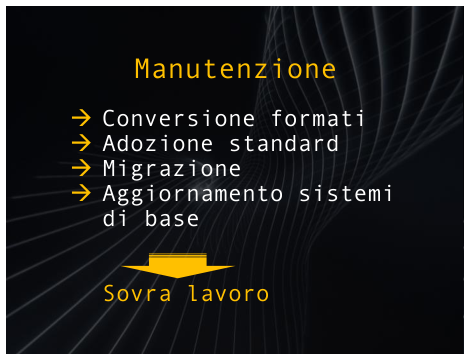
\includegraphics[width=0.50\textwidth,
                    trim=40 40 40 40, % L B R T
                    clip]
                    {images/Lez11_p05_fig_02}
  % \caption{Sommario}
  % \label{fig:Lez15_p06_fig_02}
\end{figure}
\FloatBarrier
\noindent

La manutenzione dei dati prevede sia la conversione dei formati, l'adozione di standard, cioè convertire scegliendo formati che siano standard sia per la memorizzazione, sia anche per la descrizione, quindi la scelta di convenzioni che riguardano i metadati, quindi la descrizione dei contenuti che siano stati standardizzati e anche le procedure di gestione, quindi i sistemi di riferimento per il content management.

I dati sarà opportuno che siano migrati nel tempo, quindi non vi siano restrizioni all'aggiornamento degli strumenti fisici per non incorrere in costi, in impegni di risorse umane per questo tipo di attività e in genere per l'aggiornamento dei sistemi di base, delle risorse fisiche ma anche degli strumenti di gestione di base che richiedono un sovralavoro ma portano sicuramente un vantaggio per l'affidabilità delle informazioni per la loro pulizia e per la loro corretta gestione.

Spunto di riflessione: avendo focalizzato il sistema che utilizzate per la gestione dei contenuti, descrivete le funzionalità per l'archiviazione.
Un suggerimento è di individuare, se vengono gestite con strumenti appositi i contenuti temporali e come vengono organizzati e gestiti, quali provvedimenti sono presi invece per la gestione dei contenuti a lungo termine.

\section{Collaborazione}

Collaborazione si riferisce al supporto di attività contemporanee di attori diversi che possono essere dell'interno dell'organizzazione ma anche attori che sono esterni.

Possiamo dire utenti esterni, utenti interni generici o utenti con funzionalità specifiche come gli amministratori piuttosto che la direzione che potrà peraltro avere accesso magari a informazioni di sintesi o a documenti di un certo tipo, di rilevanza strategica piuttosto che non ai dati operativi o ai contenuti, ai documenti tecnici piuttosto che più operativi gestionali.

\FloatBarrier
\begin{figure}[H]
  \centering
  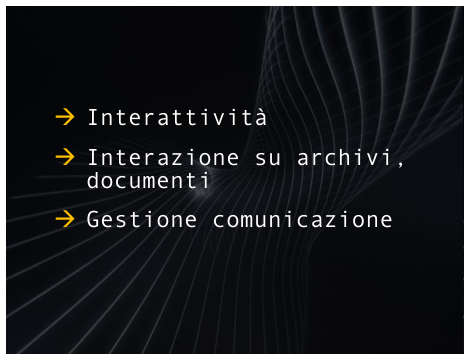
\includegraphics[width=0.50\textwidth,
                    trim=40 80 40 80, % L B R T
                    clip]
                    {images/Lez11_p05_fig_06}
  % \caption{Sommario}
  % \label{fig:Lez15_p06_fig_02}
\end{figure}
\FloatBarrier
\noindent

L'interattività si riferisce al supporto di attività che sono svolte contemporaneamente da più persone con uno stesso scopo che devono raggiungere uno stesso obiettivo supportata dalla interazione su archivi e documenti.

Interazione può essere una gestione multiutenza ma può essere anche l'adozione di basi di organizzazione di dati, di organizzazione di documenti collaborativi che permettono sia la condivisione dei dati sia la loro manipolazione e anche strumenti per la gestione della comunicazione di ogni genere, lavagne virtuali condivise piuttosto che funzioni per la condivisione dello schermo per poter mostrare le attività che si stanno svolgendo sulla propria macchina senza dover trasferire dei file o tipicamente gli screenshot, piuttosto che gestire conferenze video o conferenze audio o un'agenda che può servire sia per programmare le attività umane e quindi darsi uno scadenziario a consultazione manuale piuttosto che programmare un'agenda che venga gestita dall'eventuale modulo di gestione dei workflow e serva per attivare, temporizzare, monitorare lo svolgimento delle attività del sistema; oppure altri altri sistemi di supporto alla gestione di un progetto.

Spunto di riflessione: focalizzate il sistema che utilizzate per la gestione dei contenuti, permette un'effettiva collaborazione se la risposta è negativa che cosa modifichereste?


\section{Distribuzione} %29:24

La distribuzione chiamata anche pubblicazione dei documenti, pubblicazione dei contenuti.

La distribuzione, la pubblicazione è un'attività complessa che tocca o che interagisce con varie altre attività che riguardano la gestione dei contenuti e specificatamente la gestione, l'archiviazione e la conservazione intesa come attività di archiviazione a lungo termine.

La distribuzione o i moduli dedicati all'automatizzazione di questa attività dovranno avere una interoperabilità sintattica e semantica quindi scambio di dati ma anche intensa condivisione dei significati, dei contenuti trasportati con tutti gli elementi del sistema di gestione dei contenuti; inoltre l'attività di distribuzione avrà come fattore di valutazione positiva la molteplicità dei canali attraverso cui è permessa la pubblicazione dei dati o la distribuzione dei contenuti e quindi canali che vengono gestiti con protocolli differenti o che portano i contenuti a essere presentati su device che propongono o che richiedono presentazione di tipo differente.

\FloatBarrier
\begin{figure}[H]
  \centering
  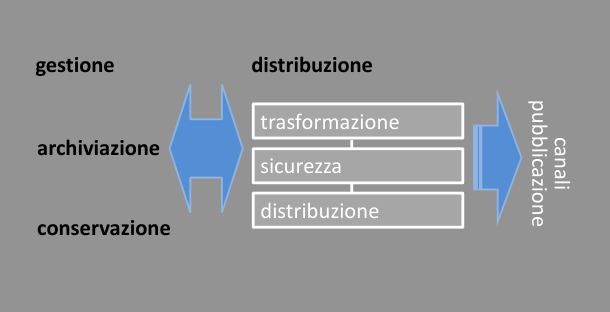
\includegraphics[width=0.50\textwidth,
                    trim=20 20 20 20, % L B R T
                    clip]
                    {images/Lez11_p06_fig_04}
  % \caption{Sommario}
  % \label{fig:Lez15_p06_fig_02}
\end{figure}
\FloatBarrier
\noindent

Vediamo questi elementi in una immagine che schematicamente mostra l'architettura funzionale della componente di pubblicazione di un content management system.
La componente di distribuzione interagisce o in altri termini prende contenuti dai moduli di gestione di archiviazione temporanea e di archiviazione permanente (conservazione).

L'invio di informazioni da parte del componente di distribuzione potrà riguardare o una richiesta sull'eventuale formato dei supporti dei contenuti che sono stati ricevuti da questi componenti o la risposta sull'avvenuta pubblicazione e sull'avvenuta diffusione multicanale dei contenuti.

La distribuzione si svolge in tre attività: trasformazione, sicurezza e distribuzione.

La distribuzione avviene attraverso molteplici canali di pubblicazione che richiederanno diversi protocolli supportati dai diversi canali e gli eventuali provvedimenti per la sicurezza per evitare che i dati siano copiati, siano eventualmente intercettati o modificati durante il loro invio se si tratta di dati sensibili; possono anche essere trasformati sia per il formato del device che li riceve sia anche per una più efficiente pubblicazione.
Nel trasferimento c'è un'eventuale compressione.

\section{Trasformazione} %35:00

\FloatBarrier
\begin{figure}[H]
  \centering
  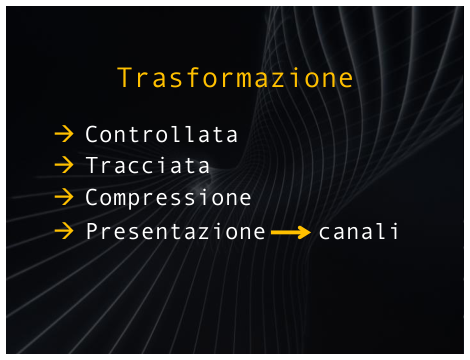
\includegraphics[width=0.50\textwidth,
                    trim=40 80 40 40, % L B R T
                    clip]
                    {images/Lez11_p06_fig_05}
  % \caption{Sommario}
  % \label{fig:Lez15_p06_fig_02}
\end{figure}
\FloatBarrier
\noindent

La trasformazione innanzitutto deve essere sempre controllata, le modifiche effettuate in fase di trasferimento di pubblicazione quindi sulla loro presentazione devono essere controllate, registrate anche per mantenere traccia di tutte le variazioni che sono state effettuate sul supporto del contenuto; non sul contenuto perché il contenuto è consolidato e approvato per la pubblicazione quindi non sarà toccato; saranno effettuate quelle modifiche di presentazione per ottimizzare la consultazione dei contenuti sui canali o attraverso i canali di diffusione che verranno utilizzati.

Inoltre i supporti potranno essere compressi ma riguarda una modifica che viene effettuata per il trasferimento ma non è una modifica permanente ma soprattutto non è una modifica strutturale, né dei contenuti, né della presentazione cioè riguarda la compressione dei dati, dei pacchetti di dati che contengono il contenuto da trasferire per ottimizzare la trasmissione del dato e verrà riportato alla forma di presentazione originaria per la sua consultazione.

La presentazione verrà specializzata per i vari canali sia con questi adeguamenti strutturali per il supporto dei contenuti sia anche per specializzare il pacchetto di informazioni che verrà effettivamente trasferito rispetto alla compatibilità col protocollo di trasmissione che sarà adottato dal canale.

\section{Sicurezza} %37:40

\FloatBarrier
\begin{figure}[H]
  \centering
  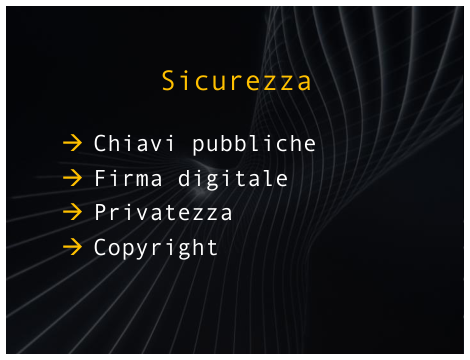
\includegraphics[width=0.50\textwidth,
                    trim=40 80 40 40, % L B R T
                    clip]
                    {images/Lez11_p06_fig_06}
  % \caption{Sommario}
  % \label{fig:Lez15_p06_fig_02}
\end{figure}
\FloatBarrier
\noindent

La sicurezza nel trasferimento dei dati è rilevante e potranno essere utilizzati metodi basati sulle chiavi pubbliche per la individuazione ed eventualmente la protezione da eventuali modifiche al supporto dei contenuti non richieste o non desiderate o per tracciare queste modifiche.

Un altro strumento potrà essere la firma digitale e questo per quanto riguarda il controllo del trasferimento dei dati quindi la eventuale protezione o memorizzazione delle modifiche che sono state tentate o effettuate durante il trasferimento.

Altri due elementi concernenti la sicurezza sono strumenti per la protezione della privatezza delle informazioni assistite eventualmente da normative riguardanti la privatezza, l'uso che si può fare dei dati trasferiti o l'uso che è non consentito dei dati quindi il livello di privacy, di riservatezza dei materiali, dei contenuti trasferiti e il rispetto dei diritti commerciali o comunque dei diritti d'autore.

\section{Canali di pubblicazione} %39:40


\FloatBarrier
\begin{figure}[H]
  \centering
  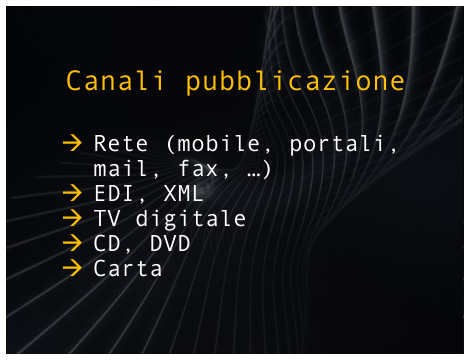
\includegraphics[width=0.50\textwidth,
                    trim=40 60 40 40, % L B R T
                    clip]
                    {images/Lez11_p07_fig_01}
  % \caption{Sommario}
  % \label{fig:Lez15_p06_fig_02}
\end{figure}
\FloatBarrier
\noindent

I canali di pubblicazione sono vari; in primo luogo mettiamo la rete internet ma solo perché attualmente è il canale più utilizzato.
La rete internet con le sue estensioni ai device mobili, ai telefoni portatili, all'utilizzo dei portali web aziendali, di mail, fax, non facciamo riferimento a un sistema specifico ma tutti gli strumenti, tutti i supporti tecnologici che possono essere dati alle nostre scelte per la nostra attività di pubblicazione di queste informazioni.

I formati potranno essere dal Electronic Data Interchange, piuttosto che l'extensible markup language, molto diffuso in ambito web.

Potranno essere trasferiti contenuti attraverso tv digitale o memorizzati per una fruizione particolare su compact disk piuttosto che dvd oppure anche stampati su carta e trasferiti per posta tradizionale.

Due spunti di riflessione: focalizzate il sistema che utilizzate per la gestione dei contenuti e descrivete come permette di distribuire le informazioni e quali sono le eventuali modifiche che apportereste.